\documentclass[10pt,letterpaper]{article}
\usepackage[utf8]{inputenc}
\usepackage[spanish, mexico]{babel}
\usepackage{graphicx}
\usepackage{subcaption}
\title{Robot seguidor de línea}
\author{Curso de introducción a LaTeX}
\begin{document}
\maketitle
Los robots seguidores de línea son robots muy sencillos, que cumplen una única misión: seguir una línea marcada en el suelo (normalmente una línea negra sobre un fondo blanco). Son considerados los "Hola mundo" de la robótica.

\section{Estructura básica}
Estos robots pueden variar desde los más básicos (van tras una línea única) hasta los robots que recorren laberintos. Todos ellos, sin embargo, poseen (por lo general) ciertas partes básicas comunes entre todos:

Sensores: un rastreador detecta la línea a seguir por medio de sensores. Hay muchos tipos de sensores que se pueden usar para este fin; sin embargo, por razones de costos y practicidad los más comunes son los sensores infrarrojos (IR), que normalmente constan de un LED infrarrojo y un fototransistor (Fig. \ref{fig:seguimiento}).

\begin{figure}[h]
	\centering
	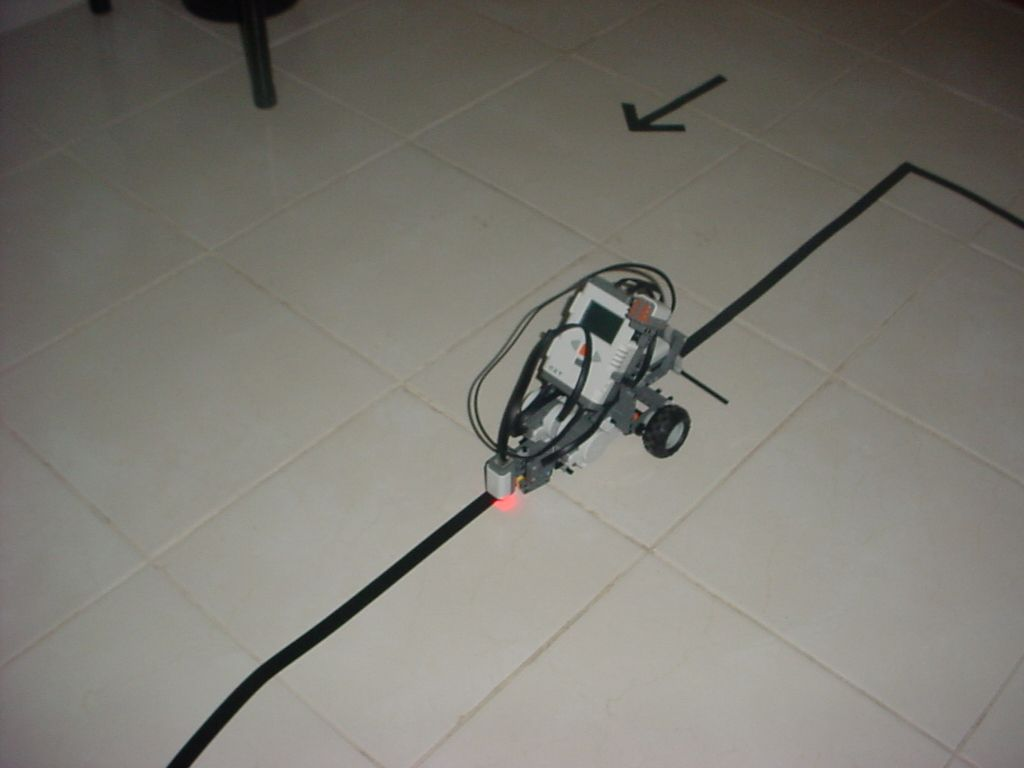
\includegraphics[width=0.7\linewidth]{fig/seguimiento}
	\caption[Seguimiento de una línea]{Seguimiento de un línea con un sensor infrarrojo}
	\label{fig:seguimiento}
\end{figure}

Motores: el robot se mueve utilizando motores. Dependiendo del tamaño, el peso, la precisión del motor, entre otros factores, éstos pueden ser de varias clases: motores de corriente continua, motores paso a paso o servomotores.

Ruedas: las ruedas del robot son movidas por los motores. Normalmente se usan ruedas de materiales anti-deslizantes para evitar fallas de tracción. Su tamaño es otro factor a tener en cuenta a la hora de armar el robot (ver fig. \ref{fig:traccion trasera}).

\begin{figure}
     \centering
     \begin{subfigure}[b]{0.45\textwidth}
             \centering
             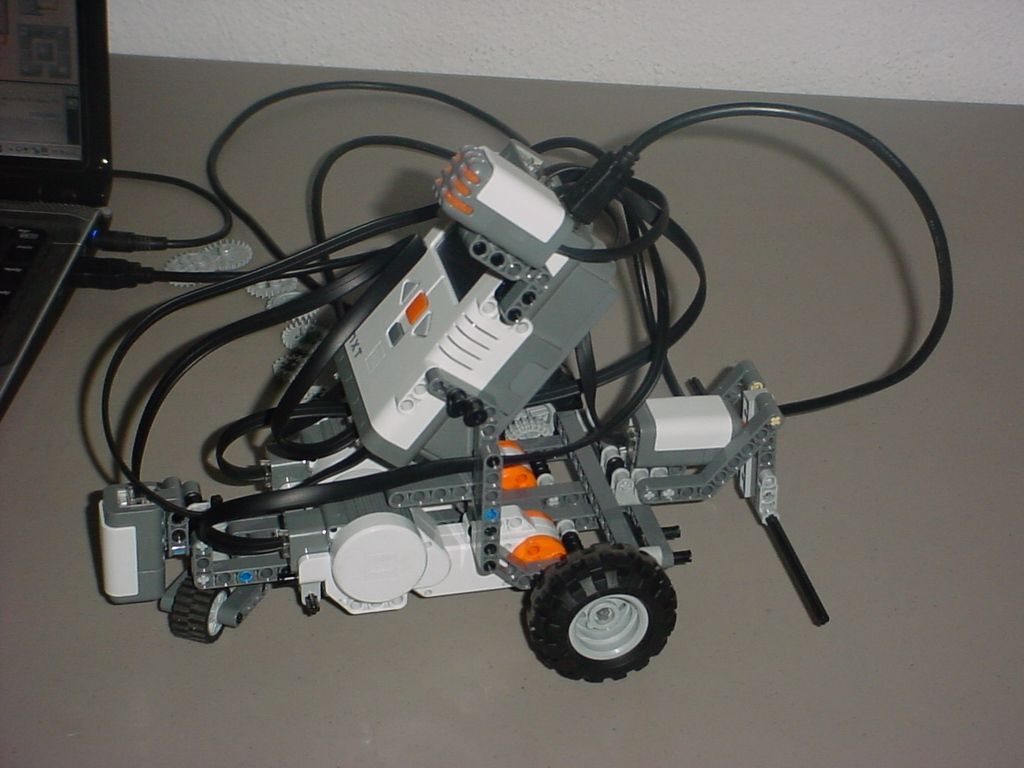
\includegraphics[width=0.7\linewidth]{fig/traccion_trasera}
             \caption[Tracción trasera]{Robot seguidor de línea con ruedas de tracción trasera}
             \label{fig:traccion trasera}
     \end{subfigure}%
     ~
     \begin{subfigure}[b]{0.45\textwidth}
             \centering
             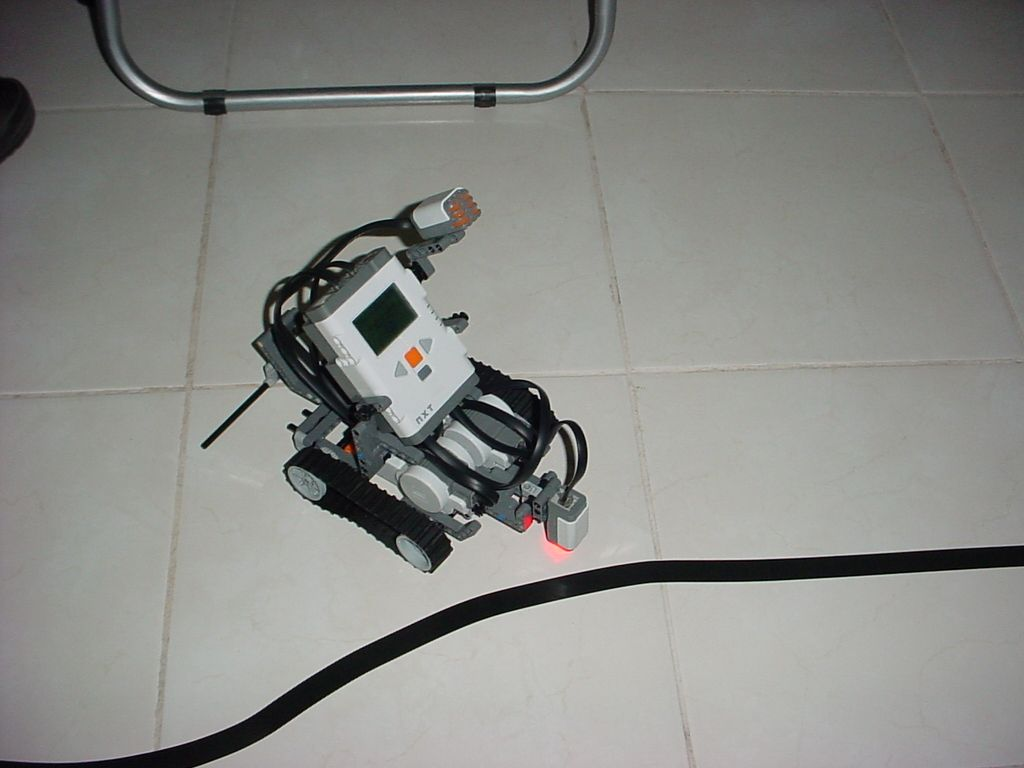
\includegraphics[width=0.7\linewidth]{fig/oruga}
             \caption[Orugas de tracción]{Robot seguidor de línea con orugas de tracción}
             \label{fig:oruga}
     \end{subfigure}
     \caption{Tipos de tracción}\label{fig:tracciones}
\end{figure}

Fuente de energía: el robot obtiene la energía que necesita para su funcionamiento de baterías o de una fuente de corriente alterna, siendo esta última menos utilizada debido a que le resta independencia al robot (ver tabla \ref{tbl:baterias}).

\begin{table}[h]
	\begin{tabular}{lp{5cm}}
		\hline Tipo de batería &  Características\\ 
		\hline
		Plomo-ácido & 6 celdas con un voltaje nominal de 2.1 V cada una  \\ 
		Gel & Alcanza su voltaje definitivo de 13.6 V \\ 
		Niquel-Cadmio (Ni-Cd) & Alcanza un voltaje de entre 1.25 V y 1.45 V \\ 
		Níquel e hidruro metálico (Ni/MH) & Similar a la de níquel-cadmio (Ni-Cd) pero no contiene cadmio (dañino con el medio ambiente) \\ 
		Iones de litio (Li-Ion) & Elevada densidad de energía \\ 
		\hline 
	\end{tabular} 
	\caption{Tipos de baterías empleadas en los robots de seguimiento de línea}
	\label{tbl:baterias}
\end{table}	

Tarjeta de control: la toma de decisiones y el control de los motores están generalmente a cargo de un microcontrolador. La tarjeta de control contiene dicho elemento, junto a otros componentes electrónicos básicos que requiere el microcontrolador para funcionar.
	
\section{Funcionamiento}
Todos los rastreadores basan su funcionamiento en los sensores. Sin embargo, dependiendo de la complejidad del recorrido, el robot debe ser más o menos complejo (y, por ende, utilizar más o menos sensores). El robot mostrado en la figura \ref{fig:seguimiento} utiliza únicamente un sensor infrarrojo.

Los rastreadores más simples utilizan 2 sensores, ubicados en la parte inferior de la estructura, uno junto al otro. Cuando uno de los dos sensores detecta el color blanco, significa que el robot está saliendo de la línea negra por ese lado. En ese momento, el robot gira hacia el lado contrario hasta que vuelve a estar sobre la línea. Esto en el caso de los seguidores de línea negra, ya que también hay seguidores de línea blanca.

Las dos maneras más comunes de armar los rastreadores son: OPAMPS (Amplificadores Operacionales), o con simples transistores trabajados en su zona de saturación. Esto dependiendo de la complejidad con la que se quiera armar el circuito. Podemos utilizar un microcontrolador para realizar las funciones de control o guardar en él la forma del recorrido por una pista. También sirve como escaneador eléctrico.
\end{document}
